\subsection{Design Overview of \gls{uefi}}
The design of UEFI is based on the following fundamental elements:

\begin{itemize}
	\item \textbf{Reuse of existing table-based interfaces} - In order to preserve investment in existing infrastructure support code, both within the OS and firmware, variety of existing specifications that are commonly implemented on platforms compatible with supported processor specifications must be implemented on platforms wishing to comply with the UEFI specification.
	\item \textbf{System partition} defines a partition and file system that are designed to allow safe sharing between multiple vendors, and for different purposes. The ability to include a separate, shareable system partition presents an opportunity to increase platform value-add without significantly growing the need for nonvolatile platform memory
	\item \textbf{Boot services} provide interfaces for devices and system functionality that
	can be used during boot time. Device access is abstracted through "handles" and
	"protocols". This facilitates reuse of investment in existing BIOS code by keeping
	underlying implementation requirements out of the specification without burdening the
	consumer accessing the device.
	\item \textbf{Runtime services} - A minimal set of runtime services is presented to ensure appropriate	abstraction of base platform hardware resources that may be needed by the OS during its	normal operations.
\end{itemize}

\begin{figure}[h]
	\centering
	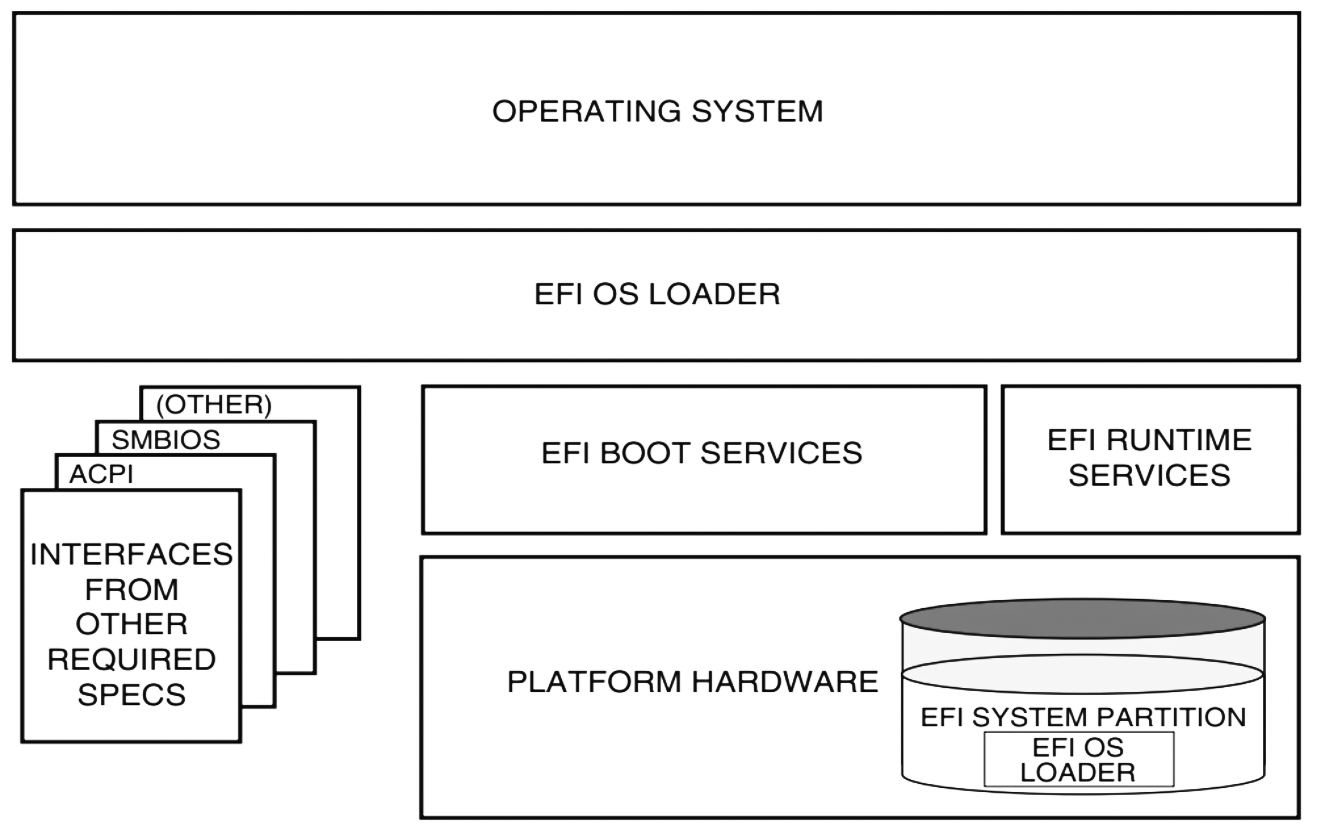
\includegraphics[width=0.8\linewidth]{design/uefi-conceptual-overview}
	\caption{UEFI Conceptual Overview}\label{fig:design-uefi-conceptual-overview}
\end{figure}

\textbf{Error! Reference source not found} illustrates the interactions of the various components of an UEFI specification-compliant system that are used to accomplish platform and OS boot.

The platform firmware can retrieve the OS loader image from the System Partition. The
specification provides for a variety of mass storage device types including disk, CD-ROM, and
DVD as well as remote boot via a network. Through the extensible protocol interfaces, it is possible
to add other boot media types, although these may require OS loader modifications if they require
use of protocols other than those defined in this document.

Once started, the OS loader continues to boot the complete operating system. To do so, it
may use the EFI boot services and interfaces defined by this or other required specifications to
survey, comprehend, and initialize the various platform components and the OS software that
manages them. EFI runtime services are also available to the OS loader during the boot phase.

\subsubsection{UEFI Driver Goals}
The UEFI Driver Model has the following goals:
\begin{itemize}
	\item \textbf{Compatible} - Drivers conforming to this specification must maintain compatibility with the EFI and the UEFI Specification. This means that the UEFI Driver Model takes advantage of the extensibility mechanisms in the UEFI Specification to add the required
	functionality.
	\item \textbf{Simple} - Drivers that conform to this specification must be simple to implement and	simple to maintain. The UEFI Driver Model must allow a driver writer to concentrate on
	the specific device for which the driver is being developed. A driver should not be
	concerned with platform policy or platform management issues. These considerations
	should be left to the system firmware.
	\item \textbf{Scalable} - The UEFI Driver Model must be able to adapt to all types of platforms. These platforms include embedded systems, mobile, and desktop systems, as well as workstations and servers.
	\item \textbf{Flexible} - The UEFI Driver Model must support the ability to enumerate all the devices, or to enumerate only those devices required to boot the required OS. The minimum device
	enumeration provides support for more rapid boot capability, and the full device enumeration provides the ability to perform OS installations, system maintenance, or system diagnostics on any boot device present in the system.
	\item \textbf{Extensible} - The UEFI Driver Model must be able to extend to future bus types as they
	are defined.

	\item \textbf{Portable} - Drivers written to the UEFI Driver Model must be portable between platforms and between supported processor architectures.
	\item \textbf{Interoperable} - Drivers must coexist with other drivers and system firmware and must do so without generating resource conflicts.
	\item \textbf{Describe complex bus hierarchies} - The UEFI Driver Model must be able to describe a variety of bus topologies from very simple single bus platforms to very complex platforms
	containing many buses of various types.

	\item \textbf{Small driver footprint} - The size of executables produced by the UEFI Driver Model must be minimized to reduce the overall platform cost. While flexibility and extensibility
	are goals, the additional overhead required to support these must be kept to a minimum to
	prevent the size of firmware components from becoming unmanageable.
	\item \textbf{Address legacy option rom issues} - The UEFI Driver Model must directly address and	solve the constraints and limitations of legacy option ROMs. Specifically, it must be
	possible to build add-in cards that support both UEFI drivers and legacy option ROMs,
	where such cards can execute in both legacy BIOS systems and UEFI-conforming latforms, without modifications to the code carried on the card. The solution must provide an evolutionary path to migrate from legacy option ROMs driver to UEFI drivers.
\end{itemize}

\subsection{\gls{uefi}/\gls{pi} Firmware Images}
\gls{uefi} and \gls{pi} specifications define the standardized format for EFI firmware storage devices (FLASH or other non-volatile storage) which are abstracted into "Firmware Volumes". Build systems must be capable of processing files to create the file formats described by the \gls{uefi} and PI specifications. The tools provided as part of the \gls{edk2} BaseTools package process files compiled by third party tools, as well as text and Unicode files in order to create UEFI or PI compliant binary image files. In some instances, where UEFI or PI specifications do not have an applicable input file format, such as the Visual Forms Representation (VFR) files used to create PI compliant IFR content, tools and documentation have been provided that allows the user to write text files that are processed into formats specified by UEFI or PI specifications.

\begin{figure}[h]
	\centering
	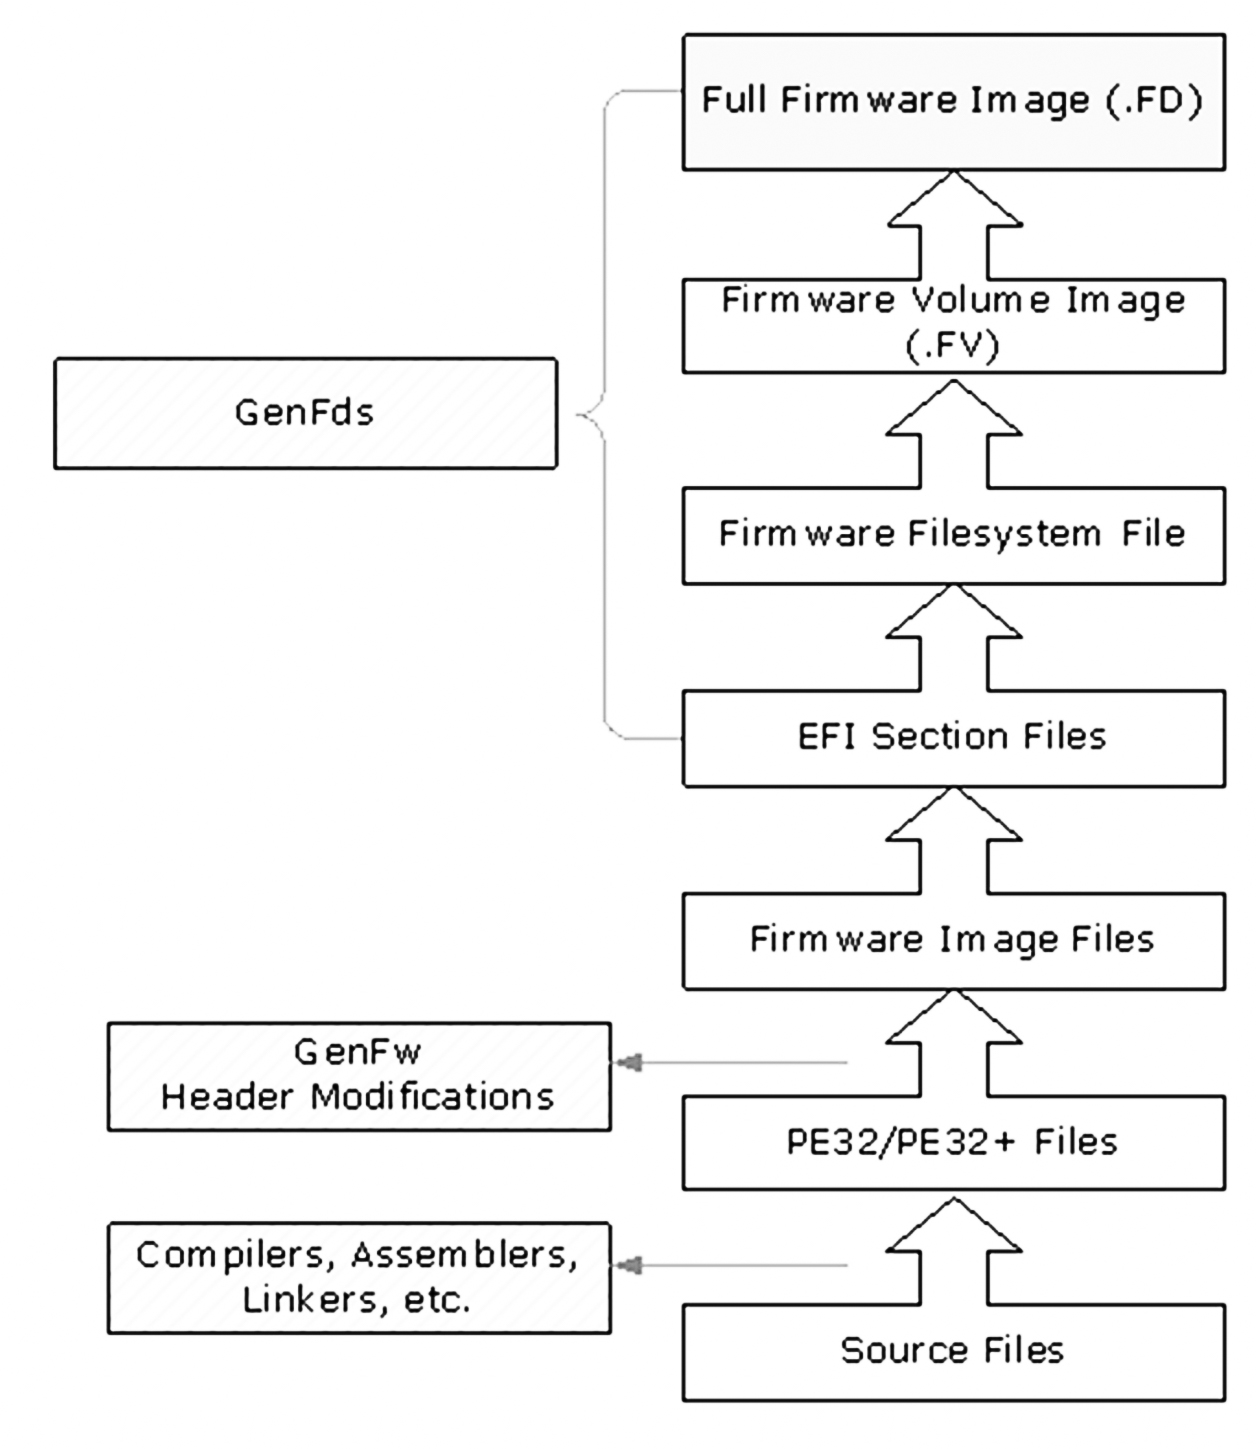
\includegraphics[width=0.8\linewidth]{design/uefi-pi-firmware-image-creation}
	\caption{UEFI/PI Firmware Image Creation}\label{fig:design-uefi-pi-firmware-image-creation}
\end{figure}

A Firmware Volume (FV) is a file level interface to firmware storage. Multiple FVs may be present in a single FLASH device, or a single FV may span multiple FLASH devices. An FV may be produced to support some other type of storage entirely, such as a disk partition or network device. For more information consult the Platform Initialization Specification, Volume 3.
In all cases, an FV is formatted with a binary file system. The file system used is typically the Firmware File System (FFS), but other file systems may be possible in some cases. Hence, all modules are stored as "files" in the FV. Some modules may be "execute in place" (linked at a fixed address and executed from the ROM), while others are relocated when they are loaded into memory and some modules may be able to run from ROM if memory is not present (at the time of the module load) or run from memory if it is available.
Files themselves have an internally defined binary format. This format allows for implementation of security, compression, signing, etc. Within this format, there are one or more "leaf" images. A leaf image could be, for example, a PE32 image for a DXE driver.

Therefore, there are several layers of organization to a full UEFI/PI firmware image. These layers are illustrated below in Figure \ref{fig:design-uefi-pi-firmware-image-creation}. Each transition between layers implies a processing step that transforms or combines previously processed files into the next higher level. Also shown in Figure \ref{fig:design-uefi-pi-firmware-image-creation} are the reference implementation tools that process the files to move them between the different layers.

\begin{figure}[h]
	\centering
	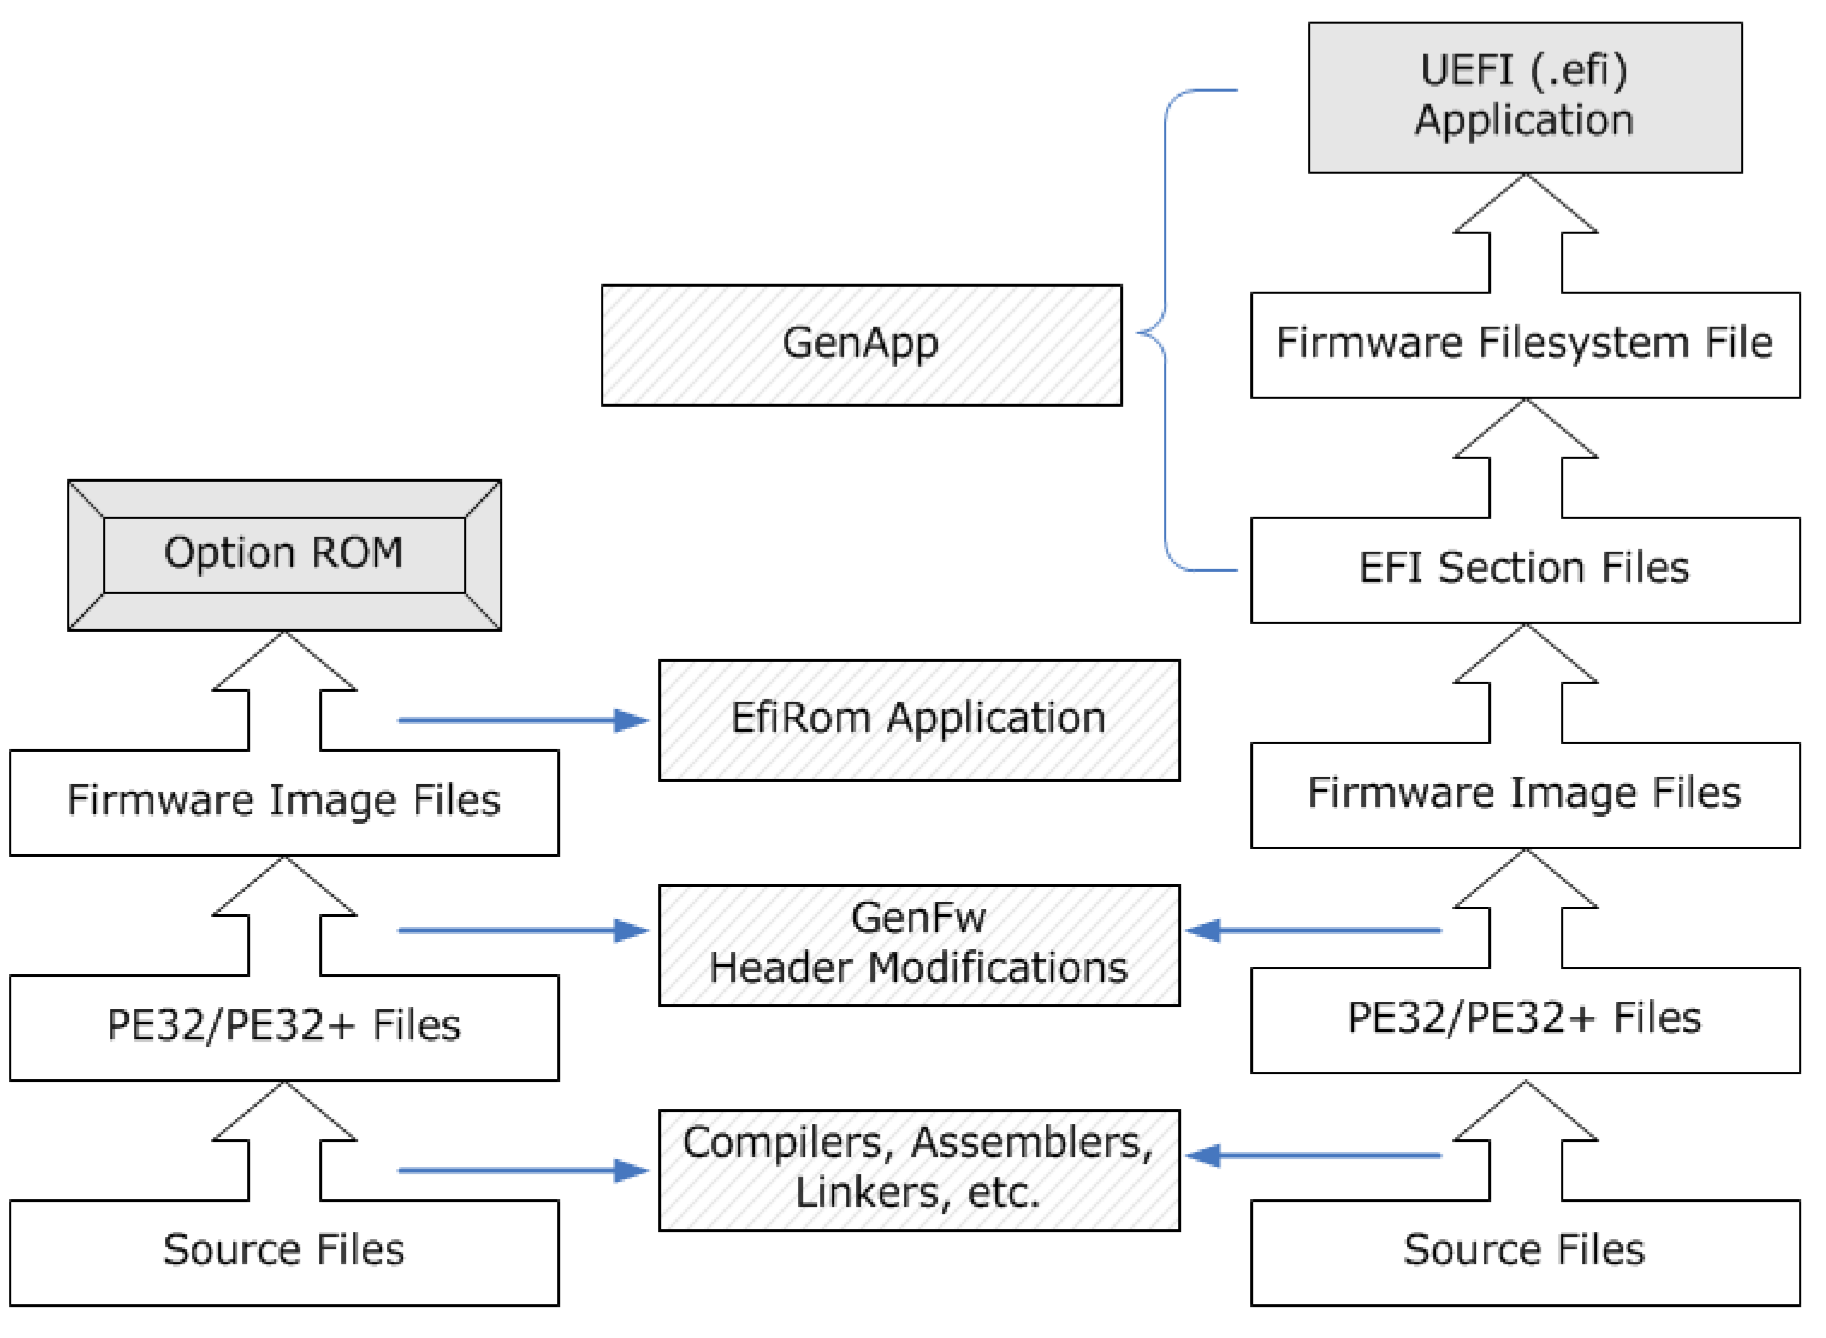
\includegraphics[width=0.9\linewidth]{design/efi-application-creation}
	\caption{UEFI/PI Firmware Image Creation}\label{fig:design-efi-application-creation}
\end{figure}


In addition to creating images that initialize a complete platform, the build process also supports creation of stand-alone UEFI applications (including OS Loaders) and Option ROM images containing driver code. Figure \ref{fig:design-efi-application-creation}, below, shows the reference implementation tools and creation processes for both of these image types

The final feature that is supported by the EDK II build process is the creation of Binary Modules that can be packaged and distributed for use by other organizations. Binary modules do not require distribution of the source code. This will permit vendors to distribute UEFI images without having to release proprietary source code.

This packaging process permits creation of an archive file containing one or more binary files that are either Firmware Image files or higher (EFI Section files, Firmware File system files, etc.). The build process will permit inserting these binary files into the appropriate level in the build stages.